\chapter{Makahiki Assessment Report}
\label{app:makahiki-assessment-report}

This appendix reports the results of the application of SGSEAM to the Makahiki framework.

We have used Makahiki to create four different Kukui Cup Energy Challenges. Kukui Cup
Energy challenges were held at the University of Hawaii (UH) in 2011 and 2012 for over
1,000 first year students living in the residence halls. Hawaii Pacific University (HPU)
held a Kukui Cup Energy challenge in Fall 2012 for about 200 students. An international
organization called the East-West Center (EWC) held a Kukui Cup Energy and Water challenge
for approximately 600 international residents living in their residence halls. Since the
halls did not have internet-enabled meters, resource consumption data had to be entered by
the game managers manually.

The successful creation of serious game challenges by three different organizations
provides evidence that Makahiki can be successfully tailored
to the needs of different organizations. First, UH and HPU used different metering
infrastructure, and EWC collected their resource data manually.  Second, while UH and HPU
challenges involved only energy consumption data, the EWC challenge involved both energy
and water consumption data. Third, the IT infrastructure at UH and HPU provided
authentication services using CAS (Central Authentication Service) and LDAP, while EWC
used the built-in Django authentication.  Fourth, the user interface was customized to
``brand'' each challenge with the logo, thematic elements, and the education contents of
the sponsoring organizations.

Besides the real world usage of Makahiki in the series of Kukui Cup challenges, we
performed in-lab assessment experiments in 2013. Makahiki was used in a serious game
development course in Spring semester of 2013 at the Information and Computer Sciences
Department of the University of Hawaii at Manoa. There were a total of 8 students who
participated in the experiments.  The participants were either senior undergraduates or
graduate students majoring in Computer Science. During the course, the students installed
Makahiki, configured and designed a serious game instance with Makahiki, and finally
developed an enhancement to the Makahiki framework. We asked the students taking the
course to voluntarily participate in the assessment experiments of Makahiki, using SGSEAM.

\section{Makahiki Player Assessment}

We applied SGSEAM to assess player effectiveness during the 2011 Kukui Cup Challenge at
the University of Hawaii at Manoa, a serious game implemented using the Makahiki
framework. There were over 1000 eligible players for this challenge, who were mostly first
year college students living in the resident halls. The challenge lasted for 3 weeks.
Makahiki recorded detailed logging data from every interaction between the players and the
website.

To assess the effectiveness of the framework for designing games that improve player literacy in sustainability, we
conducted two energy literacy surveys, one before the challenge (pre-game) and one after
the challenge (post-game). 24 players completed both surveys. Out of the total 19 energy
literacy questions, the average number of questions answered correctly is 7.54 before the
challenge, and 8.96 after the challenge. This result indicates an 18\% improvement on the
energy literacy.  We also surveyed non-players as a control condition, and found that
their literacy did not change, indicating that the improvement in player literacy was
indeed due to the game.

To assess the effectiveness of the framework for designing games that produce positive change in sustainability
behaviors, we recorded and analyzed energy consumption data before, during and after the
challenge.  Before the challenge, an energy usage baseline was established. During the
challenge, compared to the baseline, 12 out of the total 20 teams reduced their energy
consumption, with the highest reduction of 16.1\%. However, 3 teams actually increased
their energy consumption, with the highest increase of 11.7\%. Overall, the average
reduction of the 20 teams was very low---approximately 2\%.

To assess player engagement of the game, we calculated a variety of engagement
metrics. The results are shown in \autoref{fig:makahiki-engagement}:

\begin{figure}[ht!]
  \centering
  \begin{tabular}{|c|c|c|c}
    \hline
    \multicolumn{1}{|p{0.5\columnwidth}|}{\centering\tabhead{Measurement}} &
    \multicolumn{1}{|p{0.1\columnwidth}|}{\centering\tabhead{MIN}} &
    \multicolumn{1}{|p{0.1\columnwidth}|}{\centering\tabhead{AVG}} &
    \multicolumn{1}{|p{0.1\columnwidth}|}{\centering\tabhead{MAX}} \\
    \hline
    \multicolumn{1}{|p{0.5\columnwidth}|}{Participation rate} &
    \multicolumn{1}{|p{0.1\columnwidth}|}{13\%} &
    \multicolumn{1}{|p{0.1\columnwidth}|}{37\%} &
    \multicolumn{1}{|p{0.1\columnwidth}|}{74\%} \\
    \hline
    \multicolumn{1}{|p{0.5\columnwidth}|}{Number of players per day} &
    \multicolumn{1}{|p{0.1\columnwidth}|}{43} &
    \multicolumn{1}{|p{0.1\columnwidth}|}{85} &
    \multicolumn{1}{|p{0.1\columnwidth}|}{147} \\
    \hline
    \multicolumn{1}{|p{0.5\columnwidth}|}{Play time per day} &
    \multicolumn{1}{|p{0.1\columnwidth}|}{1 min} &
    \multicolumn{1}{|p{0.1\columnwidth}|}{27.7 mins} &
    \multicolumn{1}{|p{0.1\columnwidth}|}{8.5 hours} \\
    \hline
    \multicolumn{1}{|p{0.5\columnwidth}|}{submissions per day} &
    \multicolumn{1}{|p{0.1\columnwidth}|}{32} &
    \multicolumn{1}{|p{0.1\columnwidth}|}{266} &
    \multicolumn{1}{|p{0.1\columnwidth}|}{1110} \\
    \hline
    \multicolumn{1}{|p{0.5\columnwidth}|}{social interactions per day} &
    \multicolumn{1}{|p{0.1\columnwidth}|}{51} &
    \multicolumn{1}{|p{0.1\columnwidth}|}{208} &
    \multicolumn{1}{|p{0.1\columnwidth}|}{468} \\
    \hline
    \multicolumn{1}{|p{0.5\columnwidth}|}{website errors per day} &
    \multicolumn{1}{|p{0.1\columnwidth}|}{0} &
    \multicolumn{1}{|p{0.1\columnwidth}|}{0.6} &
    \multicolumn{1}{|p{0.1\columnwidth}|}{4} \\
    \hline
  \end{tabular}
  \caption{Makahiki Engagement Metrics}
  \label{fig:makahiki-engagement}
\end{figure}

The participation rate of this challenge is 37\%, which is good compared to other
sustainability challenges. Over the course of the challenge, an average player spent about
27.7 minutes per day on the website. One player spent 8.5 hours on one day. There were an
average of 266 activity submissions and 208 social interactions between players per day.

In summary, SGSEAM indicates that Makahiki can be successful in achieving
player engagement and literacy improvement. SGSEAM could not provide evidence of positive change in
behavior.

\section{Makahiki System Admin Assessment}

System admin assessment was done using an in-lab experiment.  Students in
a serious game class were tasked with installing the Makahiki system into their local
computers. In order to understand how much time it takes to install Makahiki and what
problems might be encountered, we designed a Google Form explaining the steps required to
install Makahiki. We asked the students to record the time they spent completing each step
and the problems they encountered. We also asked the students to provide feedback about
their installation experiences in the form of blog posts. \cite{csdl2-13-04} describes in detailed
the Google Form that is used in this assessment.

The results from the Google Form responses show that the average total time to successfully install
Makahiki was 1.4 hours, with a maximum time of 2 hours and the minimum time of 0.9 hour.
\autoref{fig:install-time} shows the average time for each installation step.

\begin{figure}[ht!]
  \center
  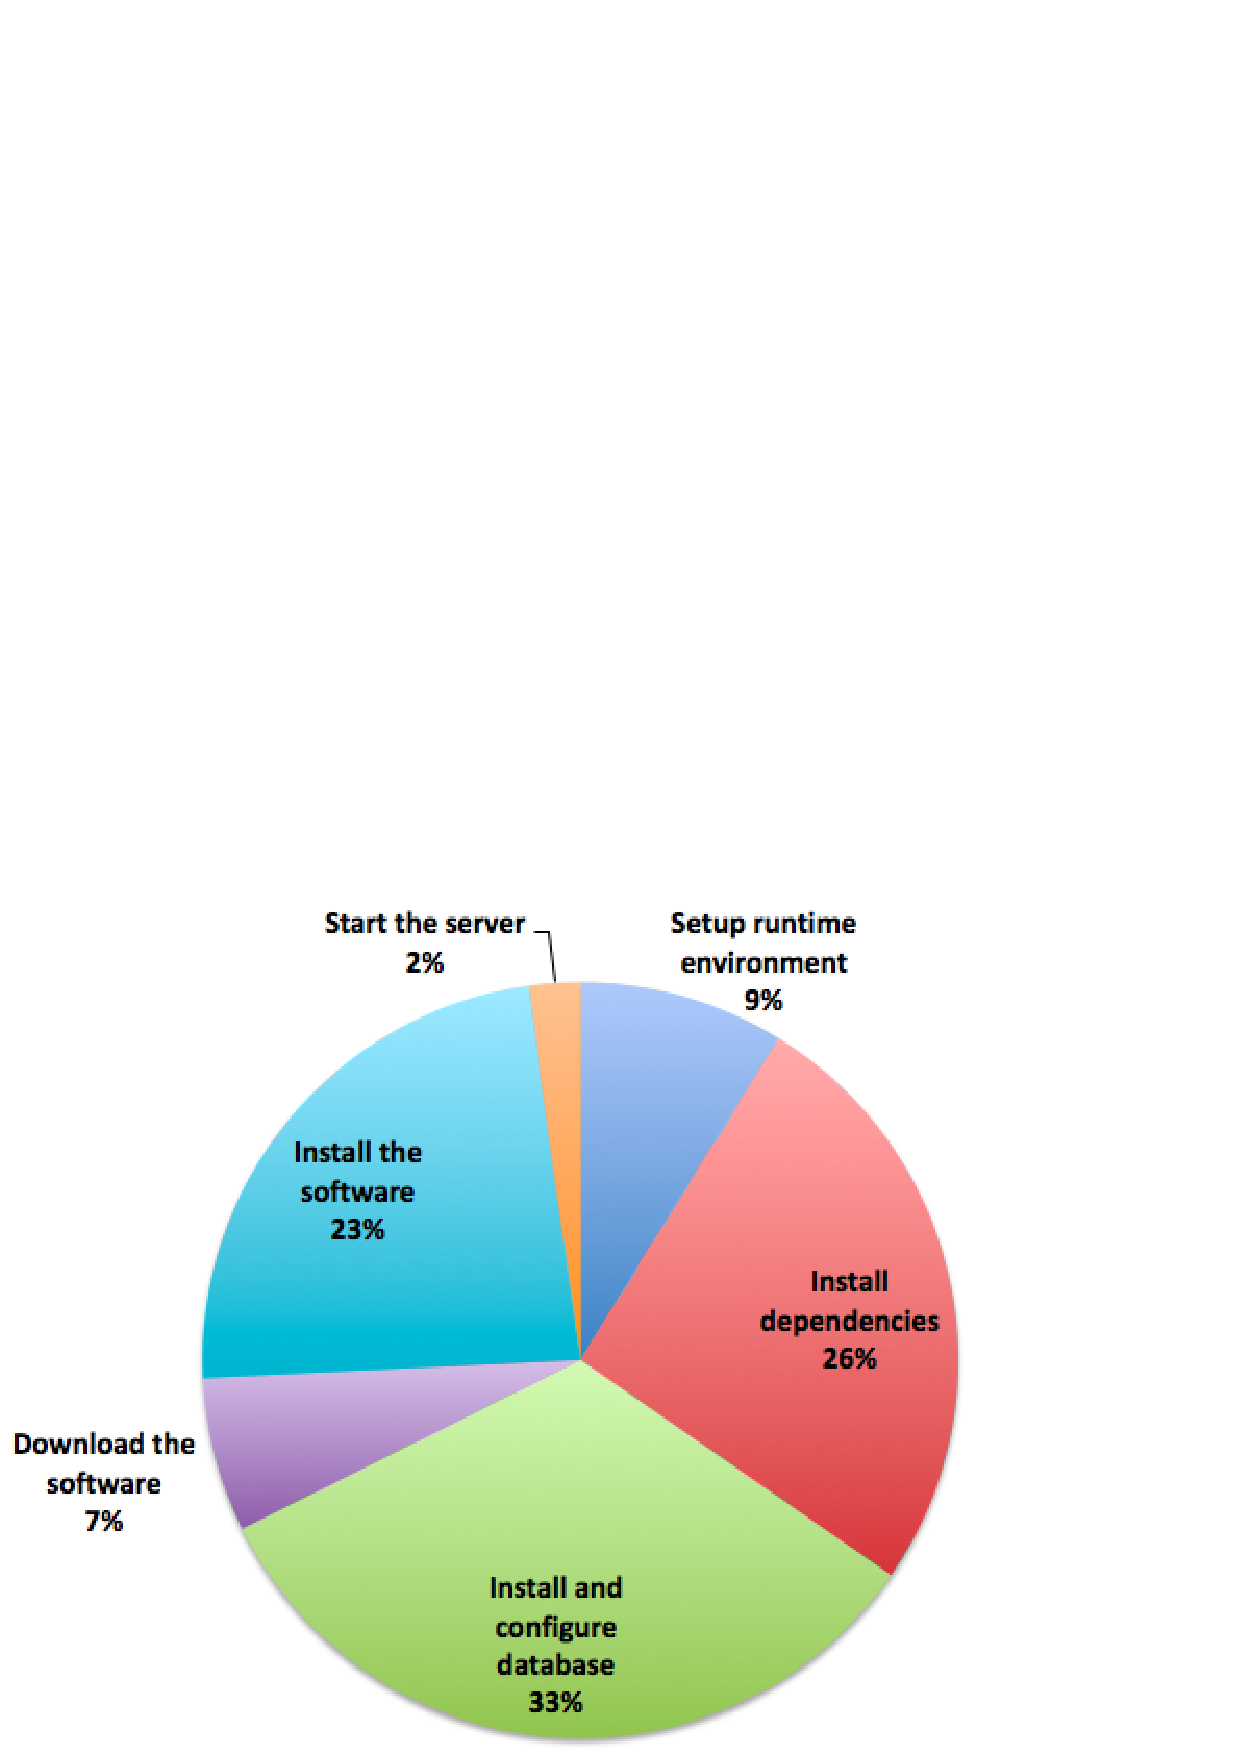
\includegraphics[width=0.7\columnwidth]{install-time}
  \caption{Average time (minutes) for installation steps (n=8)}
  \label{fig:install-time}
\end{figure}

We coded and categorized the descriptive problems reported by the students in both the Google Form
and their blog posts. \autoref{fig:makahiki-install} shows the result of the analysis from
the feedback of the 8 students that participated in the experiment.

\begin{figure}[ht!]
  \centering
  \begin{tabular}{|c|c|}
    \hline
    \multicolumn{1}{|p{0.7\columnwidth}|}{\centering\tabhead{Problem encountered}} &
    \multicolumn{1}{|p{0.2\columnwidth}|}{\centering\tabhead{Number of participants}} \\
    \hline
    \multicolumn{1}{|p{0.7\columnwidth}|}{Cannot find configuration file to edit during database installation } &
    \multicolumn{1}{|p{0.2\columnwidth}|}{4} \\
    \hline
    \multicolumn{1}{|p{0.7\columnwidth}|}{Documentation of install script is confusing about creation of the DB user} &
    \multicolumn{1}{|p{0.2\columnwidth}|}{2} \\
    \hline
    \multicolumn{1}{|p{0.7\columnwidth}|}{More parts of installation could be covered by install script} &
    \multicolumn{1}{|p{0.2\columnwidth}|}{2} \\
    \hline
  \end{tabular}
  \caption{Makahiki Installation Analysis (n=8)}
  \label{fig:makahiki-install}
\end{figure}


From the above analysis, we identified that the ``Install and configure database'' step has the
longest average time. It is also has the most participant reported problems. This reflects the issues
encountered by students during the configuration process. This assessment determines the areas for future
improvement are (1) to improve documentation on DB installation, and (2) to improve the install script to automate
more installation tasks.

In summary, SGSEAM identified database installation as a weak point in
installation.  Otherwise, SGSEAM indicates generally positive results regarding
Makahiki with respect to installation.

\section{Makahiki Game Designer Assessment}

We also used the in-lab experiment to assess the game
designer experience of Makahiki. One of the class assignments for the students in the
experiment was to design a serious game using the Makahiki framework. We asked the students
to follow specific design steps and record the time required and any problems encountered during
their design process, using a Google Form similar to the one used for the system admin
assessment. In addition, students were asked to provide feedback about their
design experiences in the form of blog posts. \cite{csdl2-13-04} describes in detailed
the Google Form that is used in this assessment.

The game designer assessment was generalized into 7 tasks corresponding to
distinct types of administrative tasks and game design planning. The time for each task is
calculated from the Google Form results.  The most time consuming task
 is "Smart Grid Game Design", which took average 107.9 minutes (56\% of total time) to complete,
 while the least time
  consuming tasks is "Raffle Game Design", which took average 7.9 minutes (7\% of total time)
  to complete.

\autoref{fig:design-time} shows the average time for each design tasks:

\begin{figure}[ht!]
  \center
  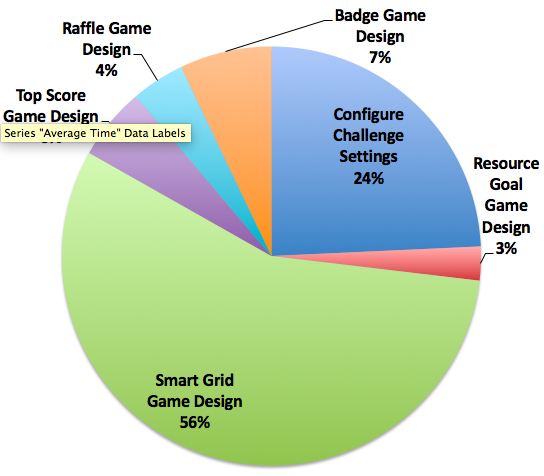
\includegraphics[width=0.7\columnwidth]{design-time}
  \caption{Average time (minutes) for design tasks (n=8)}
  \label{fig:design-time}
\end{figure}

 We aggregated the problems reported in the feedback of the 7 students that participated in the experiment.
\autoref{fig:makahiki-game-design} shows the result of the analysis:

\begin{figure}[ht!]
  \centering
  \begin{tabular}{|c|c|c|}
    \hline
    \multicolumn{1}{|p{0.7\columnwidth}|}{\centering\tabhead{Problem encountered}} &
    \multicolumn{1}{|p{0.2\columnwidth}|}{\centering\tabhead{Number of participants}} \\
    \hline
    \multicolumn{1}{|p{0.7\columnwidth}|}{Difficulty in understanding predicate system and unlock condition} &
    \multicolumn{1}{|p{0.2\columnwidth}|}{7} \\
    \hline
    \multicolumn{1}{|p{0.7\columnwidth}|}{A bug that prevented users with usernames
containing capital letters from logging in} &
    \multicolumn{1}{|p{0.2\columnwidth}|}{2} \\
    \hline
    \multicolumn{1}{|p{0.7\columnwidth}|}{A bug in the processing of Ajax queries} &
    \multicolumn{1}{|p{0.2\columnwidth}|}{1} \\
    \hline
    \multicolumn{1}{|p{0.7\columnwidth}|}{Difficulty in generating event attendance codes for game activities} &
    \multicolumn{1}{|p{0.2\columnwidth}|}{1} \\
    \hline
  \end{tabular}
  \caption{Makahiki Game Design Analysis, (n=8)}
  \label{fig:makahiki-game-design}
\end{figure}

In summary, SGSEAM revealed two shortcomings with Makahiki configuration: ``Smart
Grid Game Design'' and ``Configure Challenge Settings''. Issues encountered in ``Smart Grid Game
Design'' included 1) difficulty and lack of documentation on the predicate system used to define dependencies
between game activities, and 2) difficulty in generating event attendance codes for game activities.
Issues encountered in ``Configure Challenge Settings'' included 1) a bug in the processing of Ajax queries
caused by consecutive clicks on the same interface button, and 2) a bug that prevented users with username
containing capital letters from logging in.

\section{Makahiki Developer Assessment}

We assessed developer experience using an in-lab experiment. One of the class assignments
for the students in the experiment was to develop an enhancement to Makahiki.  This
involved setting up a development environment, following the tutorial to create a ``Hello
world'' widget using Makahiki, and finally, developing an enhancement to extend the
functionality of Makahiki.

The students were asked to submit their development source code to the
public source code repository (GitHub) and write a blog post to
discuss their efforts to complete the development activity.

All 8 students reported that the first task of creating the simple ``Hello world'' widget
was easy, while the enhancement development was hard. Only one student successfully
completed all 5 required features, while the rest successfully completed 1 or 2
features. The main problem students reported was the lack of documentation for the
development libraries. One student stated in his blog that he decided to choose Makahiki
framework to develop his own serious game because of Makahiki's features and possibility
of reducing development effort by using the framework.

In summary, SGSEAM reveals significant problems with developer efficiency.
Analysis is still ongoing regarding the specific causes of problems and how best to
address them.
